\documentclass[letterpaper,10pt]{article}
\usepackage{tabularx} % extra features for tabular environment
\usepackage{amsmath}  % improve math presentation
\usepackage{graphicx} % takes care of graphic including machinery
\usepackage{amsthm}
\usepackage{amssymb}
\usepackage{bm}
\usepackage{bbm}
\usepackage{dsfont}
\usepackage{graphicx}
\usepackage{subfigure}
\usepackage[margin=1in,letterpaper]{geometry} % decreases margins
\usepackage{cite} % takes care of citations
%\usepackage{cleveref}
\usepackage[final]{hyperref} % adds hyper links inside the generated pdf file
\hypersetup{
	colorlinks=true,       % false: boxed links; true: colored links
	linkcolor=blue,        % color of internal links
	citecolor=blue,        % color of links to bibliography
	filecolor=magenta,     % color of file links
	urlcolor=blue
}
\usepackage{blindtext}
\usepackage{url}
\usepackage{algorithm}
\usepackage{algorithmic}
\renewcommand{\algorithmicrequire}{ \textbf{Input:}} %Use Input in the format of Algorithm
\renewcommand{\algorithmicensure}{ \textbf{Output:}} %UseOutput in the format of Algorithm
%% Define a new 'leo' style for the package that will use a smaller font.
\makeatletter
\def\url@leostyle{%
	\@ifundefined{selectfont}{\def\UrlFont{\sf}}{\def\UrlFont{\small\ttfamily}}}
\makeatother
%% Now actually use the newly defined style.
\urlstyle{leo}
%\usepackage{cleveref}

%opening
\title{\textbf{Body Fat Prediction with Multiple Regression}}
\author{Zihang Wang, Yinqiu Xu, Sixu Li}

\begin{document}

\maketitle
\section{Introduction}
Body fat percentage (BFR) is believed to be one of the effective indicators of obesity \cite{relationship2015Ho}. However, accurately estimating BFP is quite expensive and time-consuming (dual energy X-ray absorptiometry \cite{anthropometric2016Lizak}), which is difficult to apply in clinical practice or daily life measurements. So, the objective of this study is to develop a simple but effective model to predict BFP. We used a real data set contained 252 male with measurements of their BFP and various anthropometric measurements and we randomly split it into training and test sets. Our model was developed on the training set based on cross-validation validation and stepwise selection, and it predicts BFP on the test set with average error about ($16.3\%$) of body fat, which is relatively accurate with limited data. In the subsequent sections, we will show how we obtain this model based on the data set we have.

\section{Data Preprocessing}
In this section, we will talk about how we began our data analysis by first preprocessing the raw data set. Basically, we preprocess our data in the following steps:
\begin{itemize}
<<<<<<< HEAD
\item[(i).] \textbf{Drop irrelevant variables:} Note that variable IDNO is just the index of each data point and variable DENSITY is not allowed to use in the prediction, so, we just dropped these two variables.
\item[(ii).] \textbf{Detect and remove outliers:} After drawing some scatter plots between body fat and each anthropometric measurements, we noticed that there are two problematic data points. One of them has $0$ BFP, which is obviously impossible, so we directly dropped it. And the other one has  height $29.5$, which is also unrealistic, but other measurements in this data point seem reasonable, so we recalculated the value of height based on the weight and BMI of this person. Besides these two points, there are also two other outliers, which have $45.1$ BFP and $48.9$ BMI correspondingly. However, these two data are reasonable in the real life, so we currently kept them and we will discuss how to deal with them later.
\item[(iii).] \textbf{Generate variables:} Note that some of the measurements don't have obvious positive or negative relationship to the BFP, for example, people with large hip circumference are not necessary to be obesity. But some ratios of different circumferences are meaningful. For instance, people with small waist hip ratio are often in the good shape. Therefore, we consider to generate several ratios such as AHR (abdomen hip ratio), WBR(wrist biceps ratio) that could be potentially used as variables in the regression analysis.
\item[(iv)] \textbf{Split data:} We randomly split the original data set into training ($80\%$) and test ($20\%$) sets, and we would develope our model on the training data and then evaluted it performance on the test data.
=======
\item[(i).] \textbf{Drop irrelevant variables:} Note that variable IDNO is just the index of each data point and variable DENSITY is not allowed to use in the prediction, so, we just dropped these two variables. 
\item[(ii).] \textbf{Data cleaning:} Firstly, we directly checked the data and we noticed that there are two people whose body fat are lower than $2$, but normally, even the body fat of a male athlete should be greater than $2\%$. So, we removed these two abnormal points. Secondly, we drew some scatter plots between body fat and each anthropometric measurements, and we noticed that there are some outliers. Data point $42$ only has height $29.5$, which is obviously unrealistic, but other measurements of it seem reasonable, so we fixed it by recalculating the value of height based on the weight and adiposity of this person. Besides, there are also two other outliers, data points $216$ and $39$, which have $45.1$ BFP and $48.9$ BMI correspondingly. However, these two data are reasonable in the real life, so we currently kept them and we will discuss how to deal with them later. Thirdly, we know that $\text{BMI} = \frac{\text{Weight}_{\text{lb}}}{\text{Height}_{\text{inch}}^2} \times 703$\footnote{The formula comes from Wikipedia \url{https://en.wikipedia.org/wiki/Body_mass_index}.}, so, we used the weight and height in the original data to calculate BMI and compared it to the adiposity we have and we found out that, for date points $163$ and $221$, the absolute value of calculated BMI minus adiposity are greater than $1$. But different from data point $42$, in $163$ and $221$, we can't tell which variable (weight, height and adiposity) is problematic, thus, we decided to drop these two data points.
\item[(iii).] \textbf{Generate new variables:} Note that some of the measurements don't have obvious positive or negative relationship to the BFP, for example, people with large hip circumference are not necessary to be obesity. But some ratios of different circumferences are meaningful. For instance, people with small waist hip ratio are often in the good shape. Therefore, we consider to generate several ratios such as AHR (abdomen hip ratio), WBR(wrist biceps ratio) that could be potentially used as variables in the regression analysis.
\item[(iv).] \textbf{Split data:} We randomly split the original data set into training ($80\%$) and test ($20\%$) sets, and we would develop our model on the training data and then evaluated it performance on the test data.
>>>>>>> 05c045d04b7386545600c37c22340a94d7f32da0
\end{itemize}


\section{Model Selection}
Note that we have many variables that could be used in the regression, which means there are tons of models that we could choose, so in this section, we will talk about how to use cross-validation to select the best model. First, we proposed several candidate models based on the stepwise regression analysis or some basic knowledge about how people usually judge they are obesity or not. In particular, for stepwise selection, we first began with different combinations of variables (one of them is learned from paper \cite{development2020Zachary}) and then using the BIC criterion to do the backward selections (this process is automatically done by R). And based on some previous researches and daily life experience, we proposed another candidate that only involves variables BMI and AHR in the regression model. After obtaining the candidate models, we did $10$-fold cross-validation on the training data and selected out the best model based on average mean absolute percentage error (MAPE)\footnote{$\text{MAPE} = \frac{1}{n}\sum_{t=1}^{n}|\frac{A_t - P_t}{A_t}|$, where $A_t$ and $P_t$ are the actual and predict value respectively.} and model complexity. Specifically, we randomly split data into $10$ equal sized subgroups. A single subgroup was retained as the validation set to calculate the MAPE and the remaining $9$ subgroups were used to run the regressions. After repeating this cross-validation process for $10$ times, we obtained an average MAPE for each candidate model and we chose the model with relatively small prediction error and less variables involved in regression.
\section{Model Diagnosis}
\section{Conclusion}



\section{Model diagnostic}
To check assumptions of a polynomial regression model, we need to check normality, homoscedasticity and outliers. Since model may contain both first and second power term of the same variable, linearity cannot be checked. We use diagnostic plots to complete this part.
First, we plot residuals and fitted values to check constant variance.
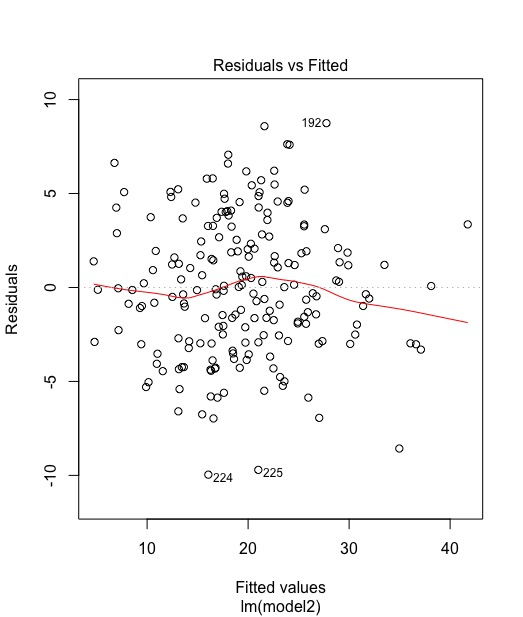
\includegraphics[scale=0.6]{ResidualVSFittedValues.jpeg}

As displayed in the above plot, the residuals behave fairly random distributed around zero. Therefore, homoscedasticity assuptions is qualified.

Secondly, we plot QQplot which can check the normality of residuals. If the points distributed almost same as the line, we can say that normality assumption is quailified.
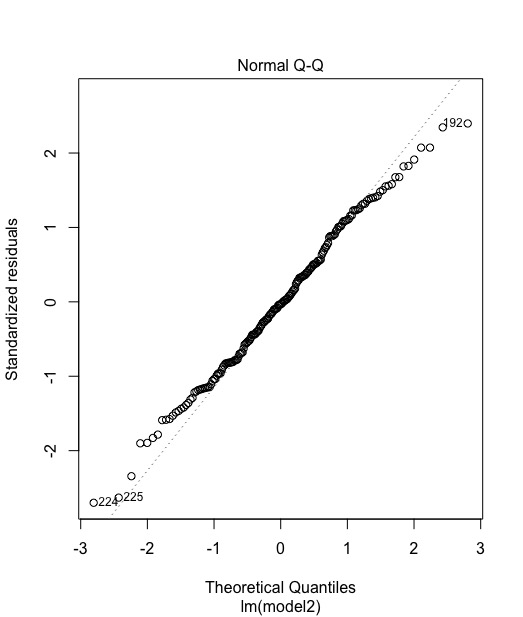
\includegraphics[scale=0.6]{normality.jpeg}

As we can see in the above plot, the QQplot behaves good. We can say that normality assumption holds.

Finally, we plot standardized residuals and leverage which is used to find possible outliers.
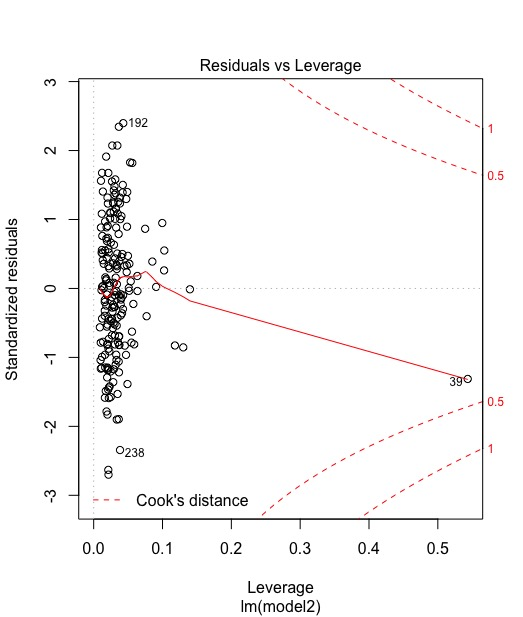
\includegraphics[scale=0.6]{outliers.jpeg}

The point 39 is suspicious. We try to fit the model again without it, the MAPE didn't be affected. Therefore, we tend to say it't not a outlier and there's no need to exclude it.

To conclude, the quadratic regression model that we present meets all assumptions. 









\bibliographystyle{acm}
\bibliography{ref}
\end{document}
